% ============================================================
% Week 1 -- Review of basic statistics and working with R
% ============================================================
\chapter{Basic Statistics, R and Data Visualisation}\label{ch:week01}

This chapter covers Week~1 of the course (Lectures 1--3). The instructor's schedule starts
with the computing environment and exploratory graphics. The linear model itself appears in
Week~2. Note that the official syllabus lists ``Review of estimation, hypothesis testing''
for Week~1, but the published Week-1 material covers R and descriptive statistics. Estimation and
testing are reviewed when they are needed (\cref{sec:L08,sec:L16}).

% ============================================================
% Lecture 1 -- Basic Statistics and Introduction to R
% ============================================================
\section{Basic Statistics and Introduction to R}\label{sec:L01}

\lectureheader{1}{z1RfnVy8Oak}{Week-1 slides \texttt{Jan26notes.pdf} (with the instructor's handwritten annotations)}

\begin{guiding*}
By the end of this lecture you should be able to:
\begin{itemize}
  \item say what R is, where it came from, and how to install R and RStudio (and what the Python equivalents are);
  \item classify data as categorical, discrete numeric or continuous numeric;
  \item describe numerical data by its \emph{centre}, \emph{spread} and \emph{shape}, and compute the mean, median, mode, variance, standard deviation and inter-quartile range;
  \item load a built-in data frame, look at it with \texttt{head}, \texttt{tail} and indexing, and make the five-number summary, histogram and scatter plots.
\end{itemize}
\end{guiding*}

\subsection{Motivation}
The course is about \emph{linear statistical models}, but every model starts with data.
Before we write down $Y = X\beta+\eps$ we have to know how to read a data set, summarise it,
and draw pictures of it. The first week therefore reviews basic descriptive statistics and
introduces the computing environment. The instructor's slides open with a light-hearted
``statutory warning'': he tends to speak quickly, and students should ask him to repeat anything
that is unclear. The same advice applies to these notes: work through every example yourself,
in the companion notebook if you like.

\subsection{The R environment}
The slides describe R as follows.
\begin{itemize}
  \item R is an open-source programming language for statistical computing. It runs on Linux, Windows and Mac~OS, and it is free. The project web page is \url{http://www.r-project.org}.
  \item R is modelled on the languages S and S-Plus. S was developed in the late 1980s at AT\&T Bell Labs.
  \item The R project was started in 1995 by Robert Gentleman and Ross Ihaka of the Statistics Department of the University of Auckland (\emph{Journal of Computational and Graphical Statistics} 5:3, 299--314, 1996). It is now maintained by the R core development team with many contributors.
  \item R is downloaded from \url{https://cloud.r-project.org}. RStudio is an \vocab{integrated development environment} (IDE) for R.
\end{itemize}
There is plenty of help available on the web, for example the R-bloggers site.

\begin{note}[Supplementary: the Python counterpart used in this book]
Throughout these notes the R demonstrations are translated into Python. The ingredients are
\texttt{numpy} (arrays and linear algebra), \texttt{pandas} (data frames),
\texttt{matplotlib}/\texttt{seaborn} (graphics), \texttt{scipy.stats} (distributions) and
\texttt{statsmodels} (linear models). The IDE is VS~Code with the Jupyter extension. Setup
instructions are in the \texttt{README.md} at the root of the project.
\end{note}

\subsection{Kinds of data}
\begin{definition}[Types of data]\label{def:L01-datatypes}
The slides distinguish three kinds of data.
\begin{enumerate}
  \item \vocab{Categorical data}: each observation belongs to one of a set of labels, for example $\{0,1\}$ or $\{A,B,\dots\}$.
  \item \vocab{Discrete numeric data}: numbers that naturally take only discrete values, for example counts.
  \item \vocab{Continuous numeric data}: numbers that can take any value in an interval, for example temperature or a stock price.
\end{enumerate}
\end{definition}
The slides refer to S.\,S.~Stevens, ``On the theory of scales of measurement'',
\emph{Science} 103 (1946), 677--680, for a finer classification of measurement data. As typical
examples of numeric data the slides mention daily temperatures and the earnings of a stock in a
stock market. Such data are visualised with histograms and boxplots.

\begin{note}[Supplementary: Stevens' scales]
Stevens' paper is best known for its four scales of measurement: \emph{nominal} (labels only),
\emph{ordinal} (labels with an order), \emph{interval} (differences are meaningful, zero is
arbitrary, e.g.\ temperature in $^\circ$F) and \emph{ratio} (a true zero, e.g.\ length). The
scale determines which summaries make sense. A mean of nominal codes is meaningless, and a
ratio of two Fahrenheit temperatures has no physical meaning.
\end{note}

\subsection{Centre, spread and shape}
For numerical data the slides single out three key features. We make each one precise. Let
$x_1,\dots,x_n$ be the data and $x_{(1)}\le\dots\le x_{(n)}$ the ordered data.

\begin{definition}[Measures of centre]\label{def:L01-centre}
\begin{itemize}
  \item The \vocab{mean} (average) is $\bar x = \frac1n\sum_{i=1}^n x_i$. If the distinct values $x_1,\dots,x_k$ occur with frequencies $f_1,\dots,f_k$ ($\sum f_i=n$), then $\bar x = \frac1n\sum_{i=1}^k f_ix_i$. This frequency form is written on the slide.
  \item The \vocab{median} is the middle ordered value: $x_{((n+1)/2)}$ if $n$ is odd, and $\tfrac12\paren{x_{(n/2)}+x_{(n/2+1)}}$ if $n$ is even.
  \item The \vocab{mode} is the most frequently occurring value.
\end{itemize}
\end{definition}

\begin{definition}[Measures of spread]\label{def:L01-spread}
\begin{itemize}
  \item The (sample) \vocab{variance} is $s^2=\frac{1}{n-1}\sum_{i=1}^n (x_i-\bar x)^2$. This is R's \texttt{var}. The \vocab{standard deviation} is $s=\sqrt{s^2}$ (R's \texttt{sd}).
  \item The \vocab{inter-quartile range} is $\mathrm{IQR}=Q_3-Q_1$, where $Q_1$ and $Q_3$ are the first and third quartiles (the $25\%$ and $75\%$ quantiles).
\end{itemize}
\end{definition}

The \emph{shape} of the data describes, for example, whether it is symmetric or skewed about its
centre, and which values are more likely than others. The instructor's sketch shows a
symmetric histogram around $0$ and an asymmetric one with a long tail. Next to the sketch he
writes that most of the data lie in an ``essential range'' from mean$-3\,$SD to mean$+3\,$SD.
The next result makes this precise for \emph{every} data set.

\begin{proposition}[Supplementary: Chebyshev's inequality for data]\label{prop:L01-cheb}
Let $\sigma_n^2=\frac1n\sum (x_i-\bar x)^2$ and suppose $\sigma_n>0$. For every $k>0$, the proportion of data points with
$\abs{x_i-\bar x}\ge k\sigma_n$ is at most $1/k^2$. In particular at least $8/9\approx 89\%$ of any
data set lies within $3\sigma_n$ of the mean.
\end{proposition}
\begin{proof}
Let $A=\{i:\abs{x_i-\bar x}\ge k\sigma_n\}$ and let $\# A$ be its size. Every term in the sum below
is non-negative, and for $i\in A$ we have $(x_i-\bar x)^2\ge k^2\sigma_n^2$. Therefore
\[
n\sigma_n^2=\sum_{i=1}^n (x_i-\bar x)^2 \;\ge\; \sum_{i\in A}(x_i-\bar x)^2\;\ge\; \#A\cdot k^2\sigma_n^2 .
\]
Dividing by $nk^2\sigma_n^2>0$ gives $\#A/n\le 1/k^2$. Taking $k=3$ gives the second statement.
\end{proof}

For roughly bell-shaped data the proportion inside mean $\pm 3\,$SD is much higher, about
$99.7\%$. That is why the instructor calls it the essential range.

\begin{proposition}[Supplementary: the mean and the median as best constants]\label{prop:L01-bestconst}
For data $x_1,\dots,x_n$,
\begin{enumerate}
  \item $c\mapsto\sum_{i=1}^n (x_i-c)^2$ is minimised uniquely at $c=\bar x$;
  \item $c\mapsto\sum_{i=1}^n \abs{x_i-c}$ is minimised at any median.
\end{enumerate}
\end{proposition}
\begin{proof}
(1) Write $x_i-c=(x_i-\bar x)+(\bar x-c)$ and expand:
\[
\sum_{i}(x_i-c)^2=\sum_i (x_i-\bar x)^2 + 2(\bar x-c)\sum_i (x_i-\bar x) + n(\bar x-c)^2 .
\]
The middle sum is $\sum_i x_i - n\bar x=0$. So $\sum(x_i-c)^2=\sum(x_i-\bar x)^2+n(\bar x-c)^2$,
which is smallest exactly when $c=\bar x$.

(2) Let $g(c)=\sum_i\abs{x_i-c}$. The function $g$ is convex and piecewise linear. At a point $c$
that is not a data value its derivative is $\#\{i:x_i<c\}-\#\{i:x_i>c\}$. This is negative while
fewer than half of the points lie below $c$ and positive once more than half do. A convex
function is minimised where its slope changes sign, which is at a median.
\end{proof}
The first identity, ``total squared deviation $=$ deviation about the mean $+$ $n\times$(distance
of the mean)$^2$'', is the simplest case of the Pythagorean decompositions behind all of least
squares. We will meet it again in \cref{sec:L08,sec:L12}.

\begin{example}[Summaries by hand]\label{ex:L01-summary}
Consider the nine observations $3,7,8,5,12,14,21,13,18$.
\end{example}
\noindent\emph{Solution.} Ordered: $3,5,7,8,12,13,14,18,21$.
\begin{itemize}
  \item Mean: $\sum x_i=101$, so $\bar x=101/9=11.2222$.
  \item Median: $n=9$ is odd, so the median is $x_{(5)}=12$.
  \item Variance: $\sum x_i^2 = 9+25+49+64+144+169+196+324+441=1421$. Hence
  $\sum (x_i-\bar x)^2=\sum x_i^2-n\bar x^2 = 1421-101^2/9 = 1421-1133.4444=287.5556$, and
  $s^2=287.5556/8=35.9444$, $s=5.9954$.
  \item Quartiles: R's default rule (\texttt{type = 7}, also NumPy's default) puts the $q$-quantile at
  ordered position $1+(n-1)q$. For $q=0.25$ this is position $3$, so $Q_1=x_{(3)}=7$. For $q=0.75$ it is
  position $7$, so $Q_3=x_{(7)}=14$. Hence $\mathrm{IQR}=7$.
  \item The five-number summary is $(\min,Q_1,\text{median},Q_3,\max)=(3,7,12,14,21)$ and the mean is $11.22$.
  The mean is below the median here: the lower tail ($3,5$) pulls it down more than the upper tail pushes it up.
\end{itemize}
These numbers are reproduced in the notebook \nb{week01/L01\_basic\_stats\_intro.ipynb}.

\subsection{Data sets and data frames}
R ships with many data sets. The command \texttt{data()} lists the installed ones, and the
instructor strongly encourages students to pick a data set and repeat the class experiments on it.

\begin{definition}[Data frame]\label{def:L01-dataframe}
A \vocab{data frame} is a rectangular collection of \emph{variables} (the columns) and
\emph{observations} (the rows).
\end{definition}

\begin{example}[The \texttt{airquality} data]\label{ex:L01-airquality}
\texttt{?airquality} describes daily air-quality measurements in New York (May--September 1973).
It is a data frame with $153$ rows and $6$ columns: \texttt{Ozone}, \texttt{Solar.R}, \texttt{Wind},
\texttt{Temp}, \texttt{Month} and \texttt{Day}. The slides use it to show the following commands.
\begin{itemize}
  \item \texttt{head(airquality)} and \texttt{tail(airquality)} show the first and the last six rows; with \texttt{n = 10}, \texttt{head} shows ten rows.
  \item \texttt{airquality[148,4]} returns \texttt{63}, the entry in row 148 and column 4 (\texttt{Temp}). The same value is \texttt{airquality\$Temp[148]}.
  \item \texttt{airquality[148,]} is the whole 148th row. \texttt{airquality[,c(1,4)]} gives the \texttt{Ozone} and \texttt{Temp} columns for all rows; \texttt{c()} builds the vector of column numbers.
  \item \texttt{summary(airquality\$Temp)} prints the five-number summary together with the mean:
  \[
  \text{Min }56,\quad Q_1\ 72,\quad \text{Median }79,\quad \text{Mean }77.88,\quad Q_3\ 85,\quad \text{Max }97.
  \]
\end{itemize}
\end{example}

\begin{note}[Indexing pitfall]
R counts from $1$, Python from $0$. In pandas, R's \texttt{airquality[148,4]} is
\texttt{aq.iloc[147, 3]} or \texttt{aq.loc[147, "Temp"]}. The value is again $63$.
\end{note}

\subsection{First plots}
The slides then make three kinds of plot.
\begin{itemize}
  \item \texttt{hist(airquality\$Temp)}: a histogram. Temperatures range from $56$ to $97$ with a peak in the high $70$s and low $80$s, and the histogram is mildly left-skewed.
  \item \texttt{plot(airquality\$Temp)}: the values plotted against their index. Because the rows are in date order, this is a time plot. It shows temperatures rising into the summer and falling in September.
  \item \texttt{plot(airquality\$Ozone, airquality\$Temp)}: a scatter plot. Days with higher ozone tend to be hotter.
  \item \texttt{plot(airquality)}: a matrix of scatter plots of every pair of variables.
\end{itemize}

\begin{figure}[ht]
\centering
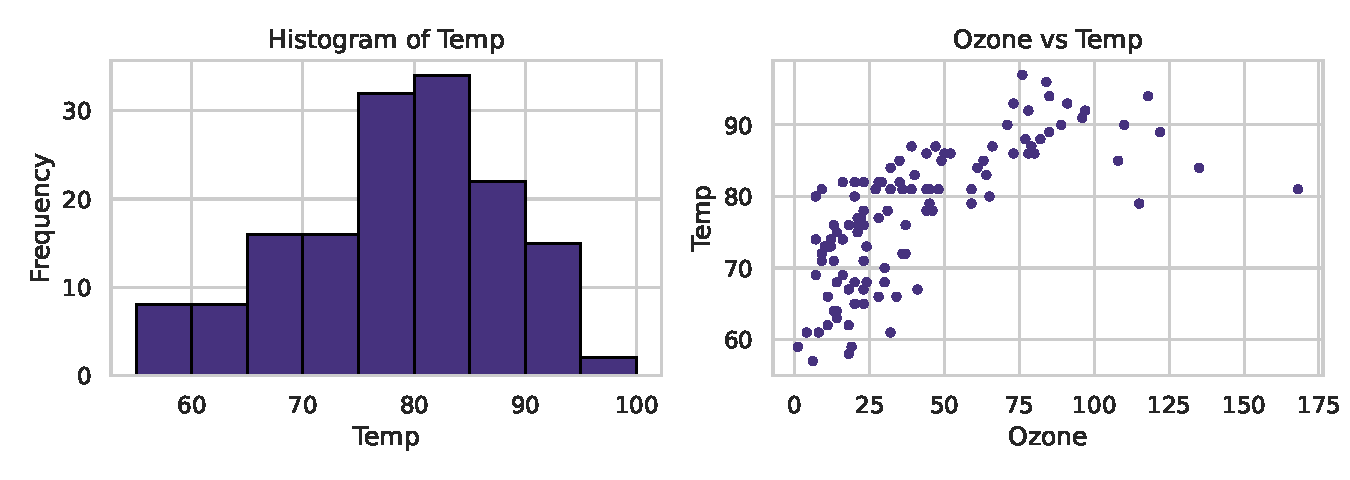
\includegraphics[width=0.95\textwidth]{figures/L01_airquality.pdf}
\caption{Histogram of \texttt{Temp} and scatter plot of \texttt{Temp} against \texttt{Ozone} (\texttt{airquality}).}
\label{fig:L01-airquality}
\end{figure}

\subsection{External packages}
R can be extended with packages. \texttt{install.packages("UsingR")} installs the package
\texttt{UsingR}, which contains many data sets, and \texttt{library("UsingR")} adds it to the
current workspace. Likewise \texttt{install.packages("tidyverse")} and
\texttt{library("tidyverse")} load \texttt{ggplot2}, the graphics system used in
\cref{sec:L02,sec:L03}.

\subsection{Computation}
The R commands of this lecture translate to Python as follows.
\begin{center}
\begin{tabular}{@{}ll@{}}\hline
R & Python (pandas / matplotlib)\\\hline
\texttt{head(airquality, n=10)} & \texttt{aq.head(10)}\\
\texttt{airquality[148,4]} & \texttt{aq.iloc[147, 3]}\\
\texttt{airquality[,c(1,4)]} & \texttt{aq.iloc[:, [0, 3]]}\\
\texttt{summary(airquality\$Temp)} & \texttt{aq.Temp.describe()}\\
\texttt{hist(airquality\$Temp)} & \texttt{plt.hist(aq.Temp)}\\
\texttt{plot(airquality)} & \texttt{pd.plotting.scatter\_matrix(aq)}\\\hline
\end{tabular}
\end{center}
Everything, including \cref{ex:L01-summary}, is in \nb{week01/L01\_basic\_stats\_intro.ipynb}.

\subsection{Summary}
\begin{itemize}
  \item R is a free language for statistics. The Python stack \texttt{pandas}/\texttt{statsmodels} does the same job in these notes.
  \item Data are categorical, discrete numeric or continuous numeric.
  \item Centre: $\bar x$, median, mode. Spread: $s^2=\frac{1}{n-1}\sum(x_i-\bar x)^2$, $s$, IQR. Shape: symmetry, skewness.
  \item $\sum(x_i-c)^2=\sum(x_i-\bar x)^2+n(\bar x-c)^2$, so the mean is the least-squares constant.
  \item A data frame has variables as columns and observations as rows. Use \texttt{head}, \texttt{tail}, indexing and \texttt{summary} to look at it, and histograms and scatter plots to picture it.
\end{itemize}

\subsection{Exercises}
\begin{problem}\label{prob:L01-1}
For the data $2,4,4,5,7,9,11$ compute the mean, median, mode, sample variance and IQR (using R's default quantile rule).
\end{problem}
\begin{problem}\label{prob:L01-2}
Show that $\sum_{i=1}^n (x_i-\bar x)^2=\sum_{i=1}^n x_i^2-n\bar x^2$.
\end{problem}
\begin{problem}\label{prob:L01-3}
Let $y_i=a+bx_i$ for constants $a,b$. Express $\bar y$, $s_y^2$ and $\mathrm{IQR}_y$ in terms of the corresponding quantities for $x$.
\end{problem}
\begin{problem}\label{prob:L01-4}
Using \texttt{airquality}, find the mean \texttt{Temp} for each month. Which month is hottest? (Use \texttt{groupby} in pandas.)
\end{problem}
\begin{problem}\label{prob:L01-5}
Give a data set of $10$ numbers in which fewer than $90\%$ of the observations lie within $2\sigma_n$ of the mean, and check that it still obeys \cref{prop:L01-cheb} with $k=2$.
\end{problem}

\subsection{Further reading}
Christensen does not cover exploratory data analysis. For this lecture see instead the
instructor's references: Verzani, \emph{simpleR} (Sections 13--15), and Wickham \& Grolemund,
\emph{R for Data Science}, Chapter~3. In Rao's \emph{Linear Statistical Inference}, the sample
moments appear in Chapter~2 (with the distribution of the sample mean and variance under
normality in Chapter~3).

% ============================================================
% Lecture 2 -- Data Visualization using ggplot2
% ============================================================
\section{Data Visualization using ggplot2}\label{sec:L02}

\lectureheader{2}{7nmwfGpgDkM}{Week-1 slides \texttt{Jan26notes.pdf}, ggplot2 part (slides on aesthetics, scaling, viridis, facets)}

\begin{guiding*}
By the end of this lecture you should be able to:
\begin{itemize}
  \item explain the idea of a \emph{grammar of graphics} and the basic \texttt{ggplot} template;
  \item map a variable to an \emph{aesthetic} (colour, shape, size) and explain what \emph{scaling} does;
  \item use colour-blind-safe \emph{viridis} palettes;
  \item split a plot into \emph{facets} with \texttt{facet\_wrap} and \texttt{facet\_grid};
  \item reproduce all of these plots in Python with \texttt{seaborn}/\texttt{matplotlib}.
\end{itemize}
\end{guiding*}

\subsection{Recap and motivation}
In \cref{sec:L01} we used R's base graphics (\texttt{hist}, \texttt{plot}). They are quick, but
each kind of plot has its own function with its own arguments. The package \texttt{ggplot2}
(loaded by \texttt{library(tidyverse)}) takes a different route: it is built on a \emph{grammar
of graphics}. The instructor's annotation sums up the benefit: ``a system for describing and
building graphs --- learn one system and apply it at many places''. In linear models we
constantly plot a response against predictors, coloured or split by a factor. This is exactly
what the grammar makes easy.

\subsection{The \texttt{mpg} data}
The running example is the tidyverse data set \texttt{mpg}. It contains observations collected
by the US Environmental Protection Agency on $38$ models of cars ($234$ rows, $11$ columns).
Two variables matter most here:
\begin{itemize}
  \item \texttt{displ}: engine displacement in litres (the car's engine size);
  \item \texttt{hwy}: fuel efficiency on the highway, in miles per gallon.
\end{itemize}
Other variables used below are \texttt{class} (type of car: 2seater, compact, midsize, minivan,
pickup, subcompact, suv), \texttt{drv} (\texttt{f} = front-wheel, \texttt{r} = rear-wheel,
\texttt{4} = four-wheel drive), \texttt{cyl} (number of cylinders) and \texttt{trans} (type of
transmission).

\subsection{The basic template}
The first plot on the slides is
\codeline{ggplot(data = mpg) + geom\_point(mapping = aes(x = displ, y = hwy))}
It shows a \emph{negative relationship between engine size and fuel efficiency}: cars with big
engines use more fuel.

\begin{definition}[The ggplot template]\label{def:L02-template}
A \texttt{ggplot2} graph is built in layers:
\begin{enumerate}
  \item \texttt{ggplot(data = <DATA>)} creates a coordinate system to which layers are added. On its own it draws an empty graph.
  \item A \vocab{geom function} such as \texttt{geom\_point()} adds a layer, here a layer of points.
  \item Each geom takes a \texttt{mapping} argument, which is always paired with \texttt{aes()}. It says which variables go on which visual channels.
\end{enumerate}
In short: \texttt{ggplot(data = <DATA>) + <GEOM\_FUNCTION>(mapping = aes(<MAPPINGS>))}.
\end{definition}

\subsection{Aesthetic mappings and scaling}
\begin{definition}[Aesthetic, mapping, scaling]\label{def:L02-aes}
An \vocab{aesthetic} is a visual property of the objects in the plot: position ($x$, $y$),
\texttt{colour}, \texttt{shape}, \texttt{size}, and so on. To \vocab{map} a variable to an
aesthetic we associate the aesthetic's name with the variable's name inside \texttt{aes()}.
\vocab{Scaling} is the step in which \texttt{ggplot2} assigns a unique level of the aesthetic
(a colour, say) to each unique level of the variable. It also adds a legend that explains the
correspondence.
\end{definition}

\begin{example}[Adding a third variable]\label{ex:L02-colour}
\texttt{ggplot(data=mpg) + geom\_point(mapping=aes(x=displ, y=hwy, colour=class))} adds the
variable \texttt{class} to the two-dimensional scatter plot by mapping it to the aesthetic
\texttt{colour}. Here the aesthetic's name is \texttt{colour} and the variable is
\texttt{class}. Scaling assigns $7$ colours to the $7$ classes, and the legend lists them.
The plot shows that most of the cars with large engines but unusually \emph{good} mileage are
\texttt{2seater}s. These are sports cars: big engines, but light bodies.
\end{example}
Other aesthetics include \texttt{shape} and \texttt{size}. The instructor notes on the slide
that one can add \texttt{shape} in exactly the same way.

\begin{figure}[ht]
\centering
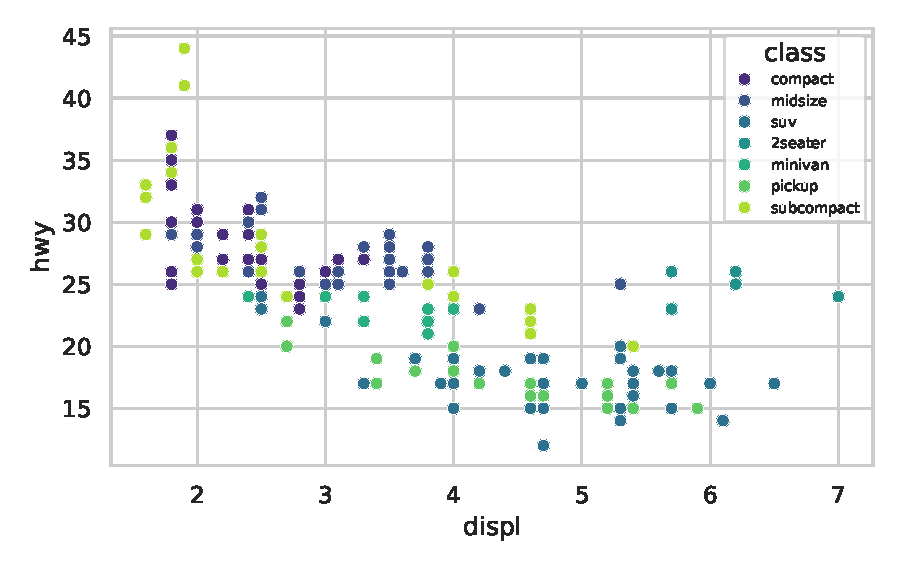
\includegraphics[width=0.7\textwidth]{figures/L02_mpg_class.pdf}
\caption{\texttt{hwy} against \texttt{displ}, coloured by \texttt{class} (viridis palette).}
\label{fig:L02-class}
\end{figure}

\begin{note}[Supplementary: mapping versus setting]
Putting \texttt{colour = class} \emph{inside} \texttt{aes()} maps a variable to colour. Putting
\texttt{colour = "blue"} \emph{outside} \texttt{aes()} just sets every point to blue. A common
beginner's mistake is \texttt{aes(colour = "blue")}. This maps a constant \emph{variable} whose
single level is the string \texttt{"blue"}, so the points get the first default colour
(pinkish-red) and a pointless legend appears.
\end{note}

\subsection{Viridis colour scales}
The viridis scales give colour maps that are \emph{perceptually uniform} in both colour and
black-and-white. They are also designed to be read correctly by viewers with common forms of
colour blindness (see \url{https://bids.github.io/colormap/}). Adding
\texttt{+ scale\_colour\_viridis\_d()} to the previous plot switches to the default viridis
palette for a discrete variable. \texttt{scale\_colour\_viridis\_d(option = "plasma")} chooses
the ``plasma'' variant.

\subsection{Facets}
Aesthetics are one way to add a variable. Another, especially useful for categorical variables,
is to split the plot into \vocab{facets}.

\begin{definition}[Facets]\label{def:L02-facets}
\texttt{facet\_wrap(\textasciitilde\ class, nrow = 2)} splits a plot by a \emph{single} variable
into subplots, each showing one subset of the data. \texttt{facet\_grid(drv \textasciitilde\ cyl)}
splits by the \emph{combination} of two variables: rows are levels of \texttt{drv}, columns are
levels of \texttt{cyl}.
\end{definition}

\begin{example}[Facets on \texttt{mpg}]\label{ex:L02-facets}
With \texttt{facet\_wrap(\textasciitilde class, nrow=2)} we get seven panels. The pickup and SUV
panels show large engines and low mileage, while the compact and subcompact panels contain the
high-mileage cars. With \texttt{facet\_grid(drv\textasciitilde cyl)} the $3\times 4$ grid shows,
for instance, that there are \emph{no} rear-wheel-drive cars with $4$ or $5$ cylinders in the
data. Those cells are empty. Facets and colour can be combined, as on the last slide of this
part:
\texttt{geom\_point(aes(colour=class)) + scale\_colour\_viridis\_d(option="plasma") + facet\_wrap(\textasciitilde class, nrow=2)}.
\end{example}

\begin{figure}[ht]
\centering
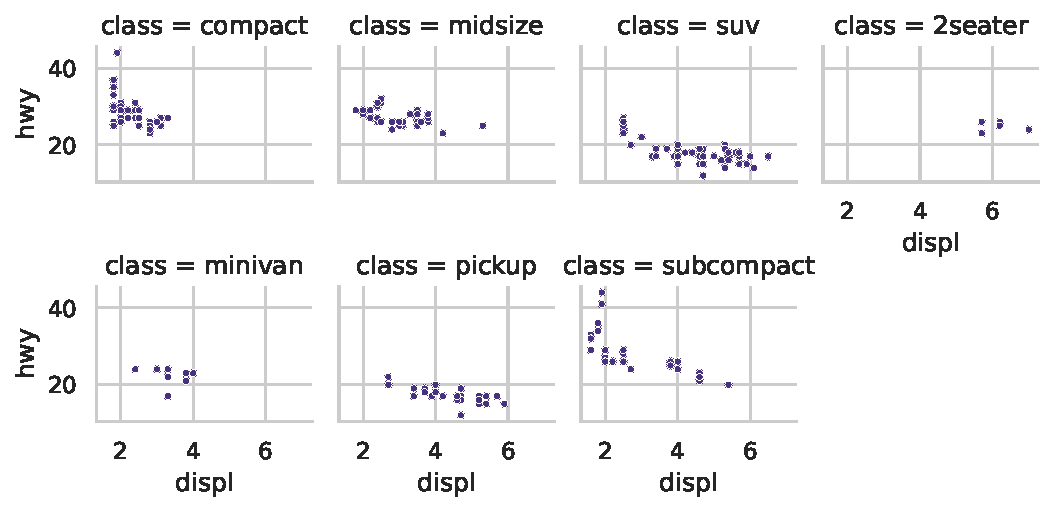
\includegraphics[width=0.95\textwidth]{figures/L02_mpg_facets.pdf}
\caption{\texttt{facet\_wrap(\textasciitilde\ class)}: one panel per class.}
\label{fig:L02-facets}
\end{figure}

\begin{note}[Supplementary: why facets matter for linear models]
In a regression of \texttt{hwy} on \texttt{displ}, the relationship could differ between
classes. For example, the slope within SUVs could differ from the slope within compacts.
Faceting by a factor is the visual version of fitting a model with a
\emph{factor $\times$ covariate interaction}. That is the analysis of covariance (ANCOVA), which
comes later in the course.
\end{note}

\subsection{Computation}
\begin{center}
\small\begin{tabular}{@{}>{\raggedright\arraybackslash}p{7.3cm}>{\raggedright\arraybackslash}p{8.3cm}@{}}\hline
R (\texttt{ggplot2}) & Python (\texttt{seaborn})\\\hline
\texttt{ggplot(mpg)+geom\_point(aes(displ,hwy))} & \texttt{sns.scatterplot(data=mpg, x="displ", y="hwy")}\\
\texttt{aes(..., colour=class)} & \texttt{hue="class"}\\
\texttt{scale\_colour\_viridis\_d()} & \texttt{palette="viridis"}\\
\texttt{option="plasma"} & \texttt{palette="plasma"}\\
\texttt{facet\_wrap(\textasciitilde class, nrow=2)} & \texttt{sns.relplot(..., col="class", col\_wrap=4)}\\
\texttt{facet\_grid(drv\textasciitilde cyl)} & \texttt{sns.relplot(..., row="drv", col="cyl")}\\\hline
\end{tabular}
\end{center}
See \nb{week01/L02\_ggplot2.ipynb}.

\subsection{Summary}
\begin{itemize}
  \item Template: \texttt{ggplot(data) + geom(mapping = aes(...))}.
  \item Aesthetics (colour, shape, size) add variables. Scaling turns variable levels into aesthetic levels and makes a legend.
  \item Viridis palettes are perceptually uniform and colour-blind safe.
  \item \texttt{facet\_wrap} splits by one variable; \texttt{facet\_grid} by two.
  \item \texttt{mpg}: engine size and highway mileage are negatively related, and the 2-seaters are the exception.
\end{itemize}

\subsection{Exercises}
\begin{problem}\label{prob:L02-1}
What goes wrong with \texttt{ggplot(mpg) + geom\_point(aes(displ, hwy, colour = "blue"))}? How do you make all points blue?
\end{problem}
\begin{problem}\label{prob:L02-2}
Map the continuous variable \texttt{cty} to \texttt{colour}. How does the legend differ from the one for \texttt{class}? Do the same in seaborn.
\end{problem}
\begin{problem}\label{prob:L02-3}
Using \texttt{facet\_grid(drv \textasciitilde\ cyl)} (or its seaborn equivalent), list the empty cells. What do they tell you about the cars in the data?
\end{problem}
\begin{problem}\label{prob:L02-4}
Count how many distinct values \texttt{class}, \texttt{drv} and \texttt{cyl} take in \texttt{mpg}. How many panels does \texttt{facet\_grid(drv \textasciitilde\ cyl)} have?
\end{problem}

\subsection{Further reading}
Wickham \& Grolemund, \emph{R for Data Science}, Chapter~3 (Data visualisation) --- the source
the instructor follows. Christensen and Rao do not cover graphics. Christensen's regression
chapters (Chapter~6 onwards) use residual plots of the kind built with these tools.

% ============================================================
% Lecture 3 -- Data Visualization using ggplot()-geoms
% ============================================================
\section{Data Visualization using ggplot()-geoms}\label{sec:L03}

\lectureheader{3}{EP8uu2k5WfA}{Week-1 slides \texttt{Jan26notes.pdf}, part ``ggplot()-geoms'' to ``layered grammar of graphics''; recap slides at the start of \texttt{Feb2.pdf}}

\begin{guiding*}
By the end of this lecture you should be able to:
\begin{itemize}
  \item explain what a \emph{geom} is and switch between \texttt{geom\_point} and \texttt{geom\_smooth};
  \item give mappings globally or per layer, and use a different data subset for one layer;
  \item explain the \emph{statistical transformation} behind a bar chart (\texttt{stat\_count}) and use \texttt{stat\_summary};
  \item use position adjustments (\texttt{dodge}) and coordinate systems (\texttt{coord\_flip}, \texttt{coord\_polar});
  \item write down the full layered grammar-of-graphics template.
\end{itemize}
\end{guiding*}

\subsection{Recap}
In \cref{sec:L02} we built scatter plots with \texttt{ggplot(data) + geom\_point(aes(...))},
added a third variable through an aesthetic, and split plots into facets. This lecture
completes the grammar. We still use the \texttt{mpg} data.

\subsection{Geoms}
\begin{definition}[Geom]\label{def:L03-geom}
A \vocab{geom} is the geometrical object that a plot uses to represent data: points, lines,
bars, boxes, and so on.
\end{definition}
The same data can be drawn with different geoms.
\begin{itemize}
  \item \texttt{ggplot(mpg) + geom\_point(aes(x = displ, y = hwy))} draws the scatter plot.
  \item \texttt{ggplot(mpg) + geom\_smooth(aes(x = displ, y = hwy))} draws a \emph{smooth curve} fitted to the same points, with a grey confidence band.
\end{itemize}
The smooth curve decreases from about $29$ mpg at $2$ litres to about $17$--$18$ mpg at
$5$ litres. The default R smoother (local \emph{quadratic} fits) then turns up slightly for the
largest engines. The upturn is caused by the 2-seaters we saw in \cref{ex:L02-colour}. The
local-\emph{linear} LOWESS used in the Python notebook flattens out instead, and it gives
about $15.5$ mpg at $6$ litres.

\begin{note}[Supplementary: what \texttt{geom\_smooth} fits]
For fewer than $1000$ observations the default smoother is \vocab{LOESS} (locally estimated
scatterplot smoothing). At each point $x_0$ it fits a low-degree polynomial to the nearby data
by \emph{weighted least squares}. Points closer to $x_0$ get larger weights. The value of that
local fit at $x_0$ is the curve's height. So even the ``model-free'' smooth curve is built from
many small least-squares fits: the subject of this course, applied locally. With
\texttt{method = "lm"} one gets the single global least-squares line instead. The instructor
uses this option in Week~5 (\cref{sec:L15}).
\end{note}

\subsection{Global and local mappings}
Mappings can be given once, in \texttt{ggplot()}, and are then inherited by every layer:
\codeline{ggplot(mpg, aes(x = displ, y = hwy)) + geom\_point(aes(color = drv)) + geom\_smooth() + scale\_colour\_viridis\_d()}
Here $x$ and $y$ are \emph{global}, while \texttt{color = drv} is \emph{local} to the point
layer. The points are coloured by drive type (4, f, r), and a single smooth curve is fitted to
all the data.

A layer can even use different data. The instructor's second version replaces the smooth by
\codeline{geom\_smooth(data = filter(mpg, drv == "4"))}
Here \texttt{filter} keeps only the four-wheel-drive cars, so the smooth curve describes only
those cars while the points still show every car.

\subsection{Bar charts and statistical transformations}
\begin{example}[Counts by class]\label{ex:L03-count}
\texttt{ggplot(mpg) + stat\_count(aes(x = class))} and
\texttt{ggplot(mpg) + geom\_bar(aes(x = class))} produce the \emph{same} bar chart. The counts
agree with \texttt{table(mpg\$class)}:
\begin{center}
\begin{tabular}{ccccccc}\hline
2seater & compact & midsize & minivan & pickup & subcompact & suv\\\hline
5 & 47 & 41 & 11 & 33 & 35 & 62\\\hline
\end{tabular}
\end{center}
The seven counts add up to $234$, the number of rows.
\end{example}

\begin{definition}[Stat]\label{def:L03-stat}
A \vocab{stat} is a \emph{statistical transformation} applied to the data before display. For a
bar chart the stat is \texttt{count}: for each level $c$ of the $x$-variable it computes
$n_c=\#\{i: x_i=c\}$ and passes the pairs $(c,n_c)$ to the bar geom. Every geom has a default
stat, and every stat has a default geom. \texttt{geom\_bar} uses \texttt{stat\_count}, and
\texttt{stat\_count} uses \texttt{geom\_bar}. This is why the two commands above are
interchangeable. \texttt{ggplot2} provides over $20$ stats (see \texttt{?stat\_bin}).
\end{definition}

\begin{example}[\texttt{stat\_summary}]\label{ex:L03-summary}
\codeline{ggplot(mpg) + stat\_summary(aes(x = class, y = hwy), fun.min = min, fun.max = max, fun = median)}
For each class this draws a point at the median highway mileage and a vertical line from the
minimum to the maximum. The values plotted are:
\begin{center}
\begin{tabular}{lccccccc}\hline
 & 2seater & compact & midsize & minivan & pickup & subcompact & suv\\\hline
min & 23 & 23 & 23 & 17 & 12 & 20 & 12\\
median & 25 & 27 & 27 & 23 & 17 & 26 & 17.5\\
max & 26 & 44 & 32 & 24 & 22 & 44 & 27\\\hline
\end{tabular}
\end{center}
Pickups and SUVs have the lowest median mileage. Compacts and subcompacts have the largest
spread: their maxima of $44$ belong to a few very efficient cars.
\end{example}

\subsection{Position adjustments and coordinate systems}
\begin{itemize}
  \item \texttt{geom\_bar(aes(x = class, fill = trans))} \emph{stacks} the bars, splitting each class bar by transmission type. The \texttt{fill} aesthetic colours the inside of the bars.
  \item \texttt{position = "dodge"} puts the pieces \emph{side by side}. This makes the counts within a class easier to compare.
  \item \texttt{coord\_flip()} swaps the axes, giving horizontal bars. This is handy for long category names.
  \item \texttt{coord\_polar()} uses polar coordinates. The bar chart becomes a ``Coxcomb'' chart.
\end{itemize}

\begin{figure}[ht]
\centering
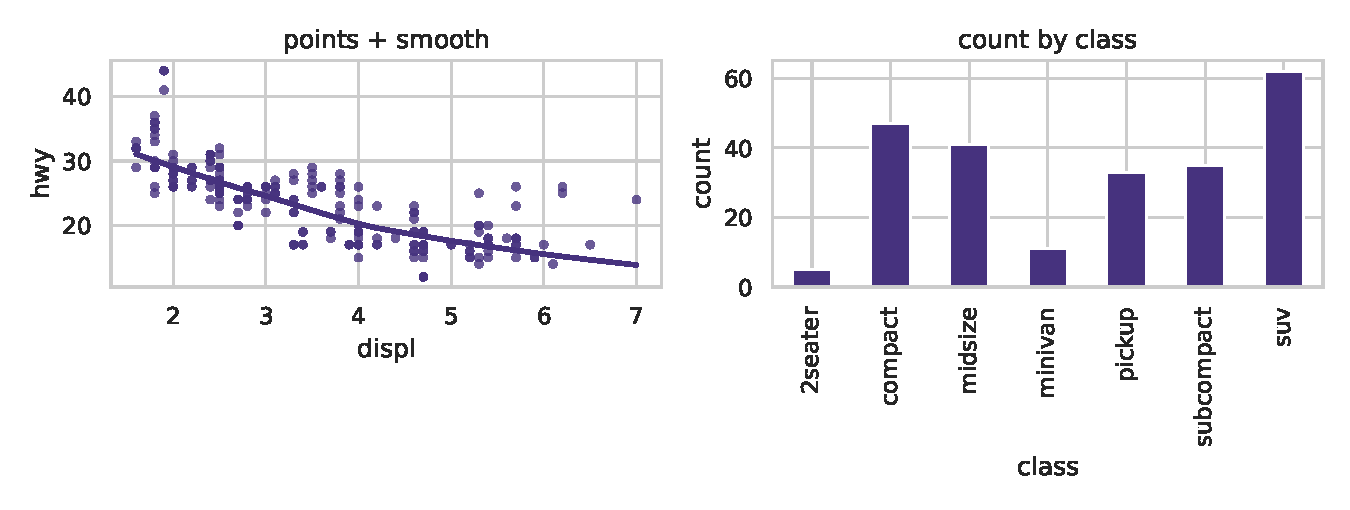
\includegraphics[width=0.95\textwidth]{figures/L03_geoms.pdf}
\caption{Left: points with a LOESS smooth. Right: the count stat behind a bar chart.}
\label{fig:L03-geoms}
\end{figure}

\subsection{The layered grammar of graphics}
\begin{definition}[Layered grammar of graphics]\label{def:L03-grammar}
Every \texttt{ggplot2} graph fits the template
\begin{center}
\begin{minipage}{0.6\textwidth}
\ttfamily
ggplot(data = <DATA>) +\\
\quad <GEOM\_FUNCTION>(\\
\quad\quad mapping = aes(<MAPPINGS>),\\
\quad\quad stat = <STAT>,\\
\quad\quad position = <POSITION>\\
\quad ) +\\
\quad <COORDINATE\_FUNCTION> +\\
\quad <FACET\_FUNCTION>
\end{minipage}
\end{center}
The seven parameters (data, geom, mapping, stat, position, coordinates, facets) are enough to
describe almost any plot.
\end{definition}
The instructor's summary annotation lists what the week covered: scatter plots, viridis colours,
bar charts, facets, geoms and coordinate systems. The recap at the start of Week~2 calls
the grammar the ``key tool in data visualisation''.

\subsection{Computation}
\begin{center}
\small\begin{tabular}{@{}>{\raggedright\arraybackslash}p{7.3cm}>{\raggedright\arraybackslash}p{8.3cm}@{}}\hline
R & Python\\\hline
\texttt{geom\_smooth()} (LOESS) & \texttt{sns.regplot(..., lowess=True)} or \texttt{statsmodels.nonparametric.lowess}\\
\texttt{filter(mpg, drv=="4")} & \texttt{mpg[mpg.drv == "4"]}\\
\texttt{geom\_bar(aes(class))} & \texttt{sns.countplot(data=mpg, x="class")}\\
\texttt{stat\_summary(fun=median, ...)} & \texttt{mpg.groupby("class").hwy} \texttt{.agg(["min", "median", "max"])}\\
\texttt{fill=trans, position="dodge"} & \texttt{sns.countplot(..., hue="trans")}\\
\texttt{coord\_flip()} & \texttt{sns.countplot(..., y="class")}\\
\texttt{coord\_polar()} & \texttt{plt.subplot(projection="polar")} with \texttt{ax.bar}\\\hline
\end{tabular}
\end{center}
See \nb{week01/L03\_ggplot\_geoms.ipynb}.

\subsection{Summary}
\begin{itemize}
  \item A geom is the object that represents data. A stat is the transformation applied first.
  \item Mappings in \texttt{ggplot()} are global; mappings in a geom are local. Each layer may use its own data.
  \item \texttt{geom\_bar} $=$ \texttt{stat\_count} $+$ bars. \texttt{stat\_summary} draws min/median/max summaries.
  \item \texttt{position="dodge"}, \texttt{coord\_flip()} and \texttt{coord\_polar()} change the layout.
  \item The template has seven parameters: data, geom, mapping, stat, position, coordinates, facets.
\end{itemize}

\subsection{Exercises}
\begin{problem}\label{prob:L03-1}
Which stat does \texttt{geom\_histogram} use, and what does it compute? How is it related to \texttt{stat\_count}?
\end{problem}
\begin{problem}\label{prob:L03-2}
Reproduce the \texttt{stat\_summary} table of \cref{ex:L03-summary} for \texttt{cty} instead of \texttt{hwy}. Which class has the largest range?
\end{problem}
\begin{problem}\label{prob:L03-3}
Explain why \texttt{geom\_smooth(method = "lm")} gives a straight line while the default gives a curve. What quantity does the \texttt{lm} line minimise?
\end{problem}
\begin{problem}\label{prob:L03-4}
Make a dodged bar chart of \texttt{drv} within each \texttt{class} in Python. Which class contains all three drive types?
\end{problem}

\subsection{Further reading}
Wickham \& Grolemund, \emph{R for Data Science}, Chapter~3 (Sections on geometric objects,
statistical transformations, position adjustments, coordinate systems and the layered grammar).


\section*{Solutions to the Exercises of Chapter~\ref{ch:week01}}
\addcontentsline{toc}{section}{Solutions to the exercises}

\paragraph{\Cref{prob:L01-1}.}
$n=7$ and $\sum x_i=42$, so $\bar x=6$. The median is $x_{(4)}=5$ and the mode is $4$.
$\sum x_i^2=312$, so $\sum(x_i-\bar x)^2=312-7\cdot 36=60$ and $s^2=60/6=10$.
Quartiles (position $1+6q$): $Q_1$ is at position $2.5$, i.e.\ $(4+4)/2=4$; $Q_3$ is at position
$5.5$, i.e.\ $(7+9)/2=8$. So $\mathrm{IQR}=4$.

\paragraph{\Cref{prob:L01-2}.}
$\sum(x_i-\bar x)^2=\sum x_i^2-2\bar x\sum x_i+n\bar x^2=\sum x_i^2-2n\bar x^2+n\bar x^2=\sum x_i^2-n\bar x^2$.

\paragraph{\Cref{prob:L01-3}.}
$\bar y=\frac1n\sum(a+bx_i)=a+b\bar x$. Then $y_i-\bar y=b(x_i-\bar x)$, so $s_y^2=b^2s_x^2$ and
$s_y=\abs{b}s_x$. The map $x\mapsto a+bx$ is monotone. For $b>0$ it keeps the order, so every
quantile transforms as $q_y=a+bq_x$. For $b<0$ it reverses the order, so $Q_1^{(y)}=a+bQ_3^{(x)}$ and
$Q_3^{(y)}=a+bQ_1^{(x)}$. The positions $1+(n-1)q$ and $1+(n-1)(1-q)$ are symmetric, so this holds
exactly for R's type-7 rule. In both cases $\mathrm{IQR}_y=\abs{b}\,\mathrm{IQR}_x$.
The shift $a$ affects only the centre.

\paragraph{\Cref{prob:L01-4}.}
\texttt{aq.groupby("Month").Temp.mean()} gives $65.55$ (May), $79.10$ (June), $83.90$ (July),
$83.97$ (August) and $76.90$ (September). August is marginally the hottest month.

\paragraph{\Cref{prob:L01-5}.}
Take eight $0$'s and two $10$'s. Then $\bar x=2$, $\sigma_n^2=(8\cdot 4+2\cdot 64)/10=16$ and
$\sigma_n=4$. The two $10$'s are at distance $8=2\sigma_n$, so only $80\%$ of the data lie strictly
within $2\sigma_n$. The proportion at distance $\ge 2\sigma_n$ is $0.2\le 1/2^2=0.25$, as
Chebyshev requires.

\paragraph{\Cref{prob:L02-1}.}
Inside \texttt{aes()}, \texttt{"blue"} is treated as a (constant) variable. ggplot maps its one
level to the first default colour and adds a legend entry ``blue''. To colour every point blue,
set the colour outside \texttt{aes()}:
\texttt{geom\_point(aes(displ, hwy), colour = "blue")}.

\paragraph{\Cref{prob:L02-2}.}
A continuous variable gets a \emph{continuous} scale. The legend is a colour bar (a gradient),
not a list of discrete keys. In seaborn, \texttt{hue="cty"} with a numeric column likewise uses a
sequential palette and shows a few representative values.

\paragraph{\Cref{prob:L02-3}.}
The cross-tabulation of \texttt{drv} against \texttt{cyl} has zeros in three cells: four-wheel
drive with $5$ cylinders, and rear-wheel drive with $4$ or $5$ cylinders. All $5$-cylinder cars
are front-wheel drive, and all rear-wheel-drive cars have $6$ or $8$ cylinders.

\paragraph{\Cref{prob:L02-4}.}
\texttt{class} has $7$ levels, \texttt{drv} has $3$ and \texttt{cyl} has $4$ ($4,5,6,8$). The grid
therefore has $3\times 4=12$ panels, three of them empty (\cref{prob:L02-3}).

\paragraph{\Cref{prob:L03-1}.}
\texttt{geom\_histogram} uses \texttt{stat\_bin}. It divides the range of the continuous $x$
variable into intervals (bins) and counts the observations in each bin. \texttt{stat\_count} counts
observations at each \emph{distinct value} of a discrete variable. \texttt{stat\_bin} is its
analogue for continuous data, where the ``values'' are the bins.

\paragraph{\Cref{prob:L03-2}.}
For \texttt{cty} (min/median/max): 2seater $15/15/16$, compact $15/20/33$, midsize $15/18/23$,
minivan $11/16/18$, pickup $9/13/17$, subcompact $14/19/35$, suv $9/13/20$. The largest range is
for subcompacts: $35-14=21$.

\paragraph{\Cref{prob:L03-3}.}
\texttt{method="lm"} fits a single global linear model $y=a+bx$ by least squares. That is, it
minimises $\sum_i (y_i-a-bx_i)^2$ over $(a,b)$ (\cref{sec:L05}). The result is necessarily a
straight line. The default LOESS fits a separate weighted least-squares polynomial near each
$x_0$, so the curve can bend.

\paragraph{\Cref{prob:L03-4}.}
\texttt{sns.countplot(data=mpg, x="class", hue="drv")}. From the cross-tabulation, only
\texttt{subcompact} contains all three drive types ($4$: 4 cars, f: 22, r: 9).
